%-------------------------designed by zcf--------------
\documentclass[UTF8,a4paper,10pt]{ctexart}
\usepackage[left=3.17cm, right=3.17cm, top=2.74cm, bottom=2.74cm]{geometry}
\usepackage{amsmath}
\usepackage{graphicx,subfig}
\usepackage{float}
\usepackage{cite}
\usepackage{caption}
\usepackage{enumerate}
\usepackage{booktabs} %表格
\usepackage{multirow}
\newcommand{\tabincell}[2]{\begin{tabular}{@{}#1@{}}#2\end{tabular}}  %表格强制换行
%-------------------------字体设置--------------
\usepackage{times} 
\newcommand{\yihao}{\fontsize{30pt}{42pt}\selectfont}           % 一号, 1.4 倍行距
\newcommand{\erhao}{\fontsize{26pt}{36pt}\selectfont}           % 一号, 1.4 倍行距
\newcommand{\xiaoer}{\fontsize{22pt}{28pt}\selectfont}          % 二号, 1.25倍行距
\newcommand{\sanhao}{\fontsize{18pt}{18pt}\selectfont}          % 小二, 单倍行距
\newcommand{\xiaosan}{\fontsize{16pt}{24pt}\selectfont}  %三号字
\newcommand{\sihao}{\fontsize{15pt}{22pt}\selectfont}        % 小三, 1.5倍行距
\newcommand{\banxiaosi}{\fontsize{14pt}{21pt}\selectfont}            % 四号, 1.5 倍行距
\newcommand{\xiaosi}{\fontsize{13pt}{19.5pt}\selectfont}    % 半小四, 1.5倍行距
\newcommand{\dawuhao}{\fontsize{12pt}{18pt}\selectfont}            % 小四, 1.5倍行距
\newcommand{\wuhao}{\fontsize{11pt}{11pt}\selectfont}       % 大五号, 单倍行距
%-------------------------章节名----------------
\usepackage{ctexcap} 
\CTEXsetup[name={,、},number={ \chinese{section}}]{section}
\CTEXsetup[name={(,)},number={\chinese{subsection}}]{subsection}
\CTEXsetup[name={,.},number={\arabic{subsubsection}}]{subsubsection}
%-------------------------页眉页脚--------------
\usepackage{fancyhdr}
\pagestyle{fancy}
\lhead{\kaishu \leftmark}
% \chead{}
\rhead{\kaishu 计算机系统设计实验报告}%加粗\bfseries 
\lfoot{}
\cfoot{\thepage}
\rfoot{}
\renewcommand{\headrulewidth}{0.1pt}  
\renewcommand{\footrulewidth}{0pt}%去掉横线
\newcommand{\HRule}{\rule{\linewidth}{0.5mm}}%标题横线
\newcommand{\HRulegrossa}{\rule{\linewidth}{1.2mm}}
%-----------------------伪代码------------------
\usepackage{algorithm}  
\usepackage{algorithmicx}  
\usepackage{algpseudocode}  
\floatname{algorithm}{Algorithm}  
\renewcommand{\algorithmicrequire}{\textbf{Input:}}  
\renewcommand{\algorithmicensure}{\textbf{Output:}} 
\usepackage{lipsum}  
\makeatletter
\newenvironment{breakablealgorithm}
  {% \begin{breakablealgorithm}
  \begin{center}
     \refstepcounter{algorithm}% New algorithm
     \hrule height.8pt depth0pt \kern2pt% \@fs@pre for \@fs@ruled
     \renewcommand{\caption}[2][\relax]{% Make a new \caption
      {\raggedright\textbf{\ALG@name~\thealgorithm} ##2\par}%
      \ifx\relax##1\relax % #1 is \relax
         \addcontentsline{loa}{algorithm}{\protect\numberline{\thealgorithm}##2}%
      \else % #1 is not \relax
         \addcontentsline{loa}{algorithm}{\protect\numberline{\thealgorithm}##1}%
      \fi
      \kern2pt\hrule\kern2pt
     }
  }{% \end{breakablealgorithm}
     \kern2pt\hrule\relax% \@fs@post for \@fs@ruled
  \end{center}
  }
\makeatother
%------------------------代码-------------------
\usepackage{xcolor} 
\usepackage{listings} 
\lstset{ 
breaklines,%自动换行
basicstyle=\small,
escapeinside=``,
keywordstyle=\color{ blue!70} \bfseries,
commentstyle=\color{red!50!green!50!blue!50},% 
stringstyle=\ttfamily,% 
extendedchars=false,% 
linewidth=\textwidth,% 
numbers=left,% 
numberstyle=\tiny \color{blue!50},% 
frame=trbl% 
rulesepcolor= \color{ red!20!green!20!blue!20} 
}
%------------超链接----------
\usepackage[colorlinks,linkcolor=black,anchorcolor=blue]{hyperref}
%------------------------TODO-------------------
\usepackage{enumitem,amssymb}
\newlist{todolist}{itemize}{2}
\setlist[todolist]{label=$\square$}
% for check symbol 
\usepackage{pifont}
\newcommand{\cmark}{\ding{51}}%
\newcommand{\xmark}{\ding{55}}%
\newcommand{\done}{\rlap{$\square$}{\raisebox{2pt}{\large\hspace{1pt}\cmark}}\hspace{-2.5pt}}
\newcommand{\wontfix}{\rlap{$\square$}{\large\hspace{1pt}\xmark}}
%------------------------水印-------------------
\usepackage{tikz}
\usepackage{xcolor}
\usepackage{eso-pic}

\newcommand{\watermark}[3]{\AddToShipoutPictureBG{
\parbox[b][\paperheight]{\paperwidth}{
\vfill%
\centering%
\tikz[remember picture, overlay]%
  \node [rotate = #1, scale = #2] at (current page.center)%
    {\textcolor{gray!80!cyan!30!magenta!30}{#3}};
\vfill}}}

%———————————————————————————————————————————正文———————————————————————————————————————————————
%----------------------------------------------
\begin{document}
\begin{titlepage}
    \begin{center}
    \includegraphics[width=0.8\textwidth]{NKU.png}\\[1cm]    
    \textsc{\Huge \kaishu{\textbf{南\ \ \ \ \ \ 开\ \ \ \ \ \ 大\ \ \ \ \ \ 学}} }\\[0.9cm]
    \HRule \\[0.9cm]
    { \LARGE \bfseries ShouChun OS设计文档}\\[0.4cm]
    \HRule \\[2.0cm]
    \centering
    \textsc{\LARGE \kaishu{\ \ 队伍名称:寿春队}}\\[0.5cm]
    \textsc{\LARGE \kaishu{\ \ 队伍成员:林坤\quad 邹先宇\quad 郑博月}}\\[0.5cm]
    \textsc{\LARGE \kaishu{\ \ 指导老师:宫晓利\quad 张金}}\\[0.5cm]
    \vfill
    {\Large \today}
    \end{center}
\end{titlepage}
%----------------------------------------------------------------
% 目录
\tableofcontents
%----------------------------------------------------------------
\newpage

【文档情况】

前文尚未核对

正在写内存管理最后部分(但内存管理优化方法暂时没想好怎么写),
到7.28上午预计大致完成文件系统部分

而后根据系统实现写OS设计小节

最后核对文档内容作图

\newpage
\watermark{60}{10}{NKU}
\setcounter{page}{1}

\section{概述}

\textbf{ShouChun OS}是面向\textbf{2022全国大学生计算机系统能力大赛操作系统设计赛(https://os.edu
cg.net/2022CSCC)}的比赛要求进行设计与实现的,该系统为使用\textbf{C语言}进行实现、基于RISCV的\textbf{多核操作系统},可运行在QEMU(RISCV64 System)
模拟器以及HiFive Unmatched开发板上。

在比赛之前,小队成员系统学习分析了清华大学的uCore教学实验,并进行了操作系统相关知识的学习。
结合比赛要求与团队能力情况,我们决定将清华大学陶天骅所开发的\textbf{uCore-SMP(https://github.com/TianhuaTao/uCore-SMP)}
源代码作为开发基础,移植到HiFive Unmatched开发板上进行完善与改进。

\subsection{项目背景及意义}

操作系统作为计算机系统的管家,为用户程序提供了一个简单清晰的计算机模型。由于操作系统所管理的计算机系统较为复杂,
但又对于理解计算机运行原理来说至关重要,所以在本科教学过程中,操作系统是一个困难而重要的学科。

\textbf{南开大学十分重视操作系统知识的教授},故十分鼓励学生进行课程知识学习之外的拓展与实践。
本科学习阶段注重于基本理论知识的学习,由于课时限制的原因,
操作系统课程停留在单核操作系统阶段,学生初步了形成一个较为系统清晰的知识体系。
然而,现代计算机硬件技术发展飞速,多核以及异构架构的硬件日新月异,操作系统作为
软件运行中重要的一环也需要不断更新拓展。

因此,理论知识也应当不断更新,与时俱进,课程之外的学习实践十分重要。
\textbf{以赛促学},于是项目小组决定在参加操作系统大赛的过程中不断学习,
拓展理论知识,并通过编程实践提高动手能力和计算机系统设计能力,锻炼自身解决复杂工程问题的能力。


\subsection{国内外研究现状}

\subsection{项目工作概述}

\subsubsection{开发框架}

该项目的开发均基于\textbf{uCore-SMP(清华大学,陶天骅)}。uCore-SMP大量引用
了MIT的xv6(https://github.com/mit-pdos/xv6-riscv),但是同时也存在许多不同之处。相比于xv6,uCore-SMP
具有不同的系统调用、不同的内存布局、不同的代码风格等等,此外uCore-SMP使用了一个SBI来做硬件的抽象化。
经过学习研究后,项目组将uCore-SMP与比赛要求进行了比较,发现\textbf{需要实现更多的系统调用,并且需要调整文件系统、进程管理、内存管理等
功能的实现}。

uCore-SMP是基于riscv64而实现的操作系统,支持多处理器工作,符合比赛方所要求的开发板条件。同时
uCore-SMP主要使用了C语言进行开发,更易上手。\textbf{于是项目小组选择了uCore-SMP作为基础进行开发},
从而将其应用于不同于原K210开发板的HiFive Unmatched开发板上,从而满足比赛所需求的功能。
\subsubsection{实现功能}

本项目主要是面对操作系统大赛的要求进行开发的,比赛要求实现\textbf{需要实现的功能}如下:

\begin{itemize}
  \item 启动和系统初始化
  \item 内存管理
  \item 进程管理和中断异常机制
  \item 系统调用
  \item FAT32文件系统
  \item 命令解释程序
\end{itemize}

\subsubsection{开发环境}

项目开发过程中使用的硬件模拟器为QEMU。本项目选择的硬件实验设备为HiFive Unmatched开发板,其主要参数如下:

(1) CPU: 64位SiFive FU740 SoC,集成四个1.5GHz U74-MC 内核 + 一个 S7 嵌入式内核

(2)内存:16GB DDR4 RAM

(3)板载32MB SPI闪存芯片,提供了 4×USB 3.2 Gen 1 端口、一个 PCI Express x16 插槽(x8 速率)、
一个 NVME M.2 插槽、microSD 读卡器、以及千兆以太网

\section{任务分析总结}

本项目开发所基于的uCore-SMP是基于MIT的xv6进一步实现的、支持多核的操作系统。但是其原支持硬件平台为K210开发板,
且只实现了部分系统调用。为成功移植uCore-SMP到HiFive Unmatched开发板,并且实现比赛所要求实现的功能,需要对原代码
进行修改调整。从比赛要求所需要的\textbf{系统调用}出发进行需求的分析总结,总的来说需要的工作为:

\begin{itemize}
  \item 实现SD卡驱动
  \item 参照Linux操作系统进行FAT32文件系统的移植
  \item 调整文件管理结构
  \item 实现加载文件使用的loader
  \item 实现系统调用,根据要求调整内存、进程和文件相关代码
  \item 实现静态链接与动态链接
\end{itemize}

按照比赛所设定的阶段,任务也可以按照阶段进行划分,具体表现为不同阶段实现的系统调用:

【这里需要改动】
\subsection{初赛阶段}

经任务分析和编程实现,初赛阶段完成的系统调用及调用号宏定义如下(比赛要求中的39及40系统调用尚未实现):

\begin{lstlisting}[title=实现的系统调用及其系统调用号,frame=trbl,language={C}]
  #define SYS_getcwd 17
  #define SYS_dup 23
  #define SYS_dup3 24
  #define SYS_mknod 33
  #define SYS_mkdirat 34
  #define SYS_unlinkat 35
  #define SYS_linkat 37
  #define SYS_umount2 39//TODO
  #define SYS_mount 40//TODO
  #define SYS_chdir 49
  #define SYS_openat 56
  #define SYS_close 57
  #define SYS_pipe2 59
  #define SYS_getdents64 61
  #define SYS_read 63
  #define SYS_write 64
  #define SYS_fstat 80
  #define SYS_exit 93
  #define SYS_waitpid 95
  #define SYS_sched_yield 124
  #define SYS_kill 129
  #define SYS_setpriority 140
  #define SYS_getpriority 141
  #define SYS_times 153
  #define SYS_uname 160
  #define SYS_gettimeofday 169
  #define SYS_settimeofday 170
  #define SYS_getpid 172
  #define SYS_getppid 173
  #define SYS_sysinfo 179
  #define SYS_brk 214
  #define SYS_munmap 215
  #define SYS_clone 220
  #define SYS_execve 221
  #define SYS_mmap 222
  #define SYS_wait4 260
  #define SYS_execv 281
  #define SYS_sharedmem 282
  #define SYS_spawn 400
  #define SYS_mailread 401
  #define SYS_mailwrite 402
\end{lstlisting}

\subsection{决赛阶段}

决赛使用了musl和libc-test作为赛题,需要额外实现动态链接的功能。这需要我们
继续对系统调用进行完善。

\section{系统框架设计}

\subsection{整体框架}

ShouChun OS的设计框架图如下所示:

\begin{figure}[H]
  \centering
  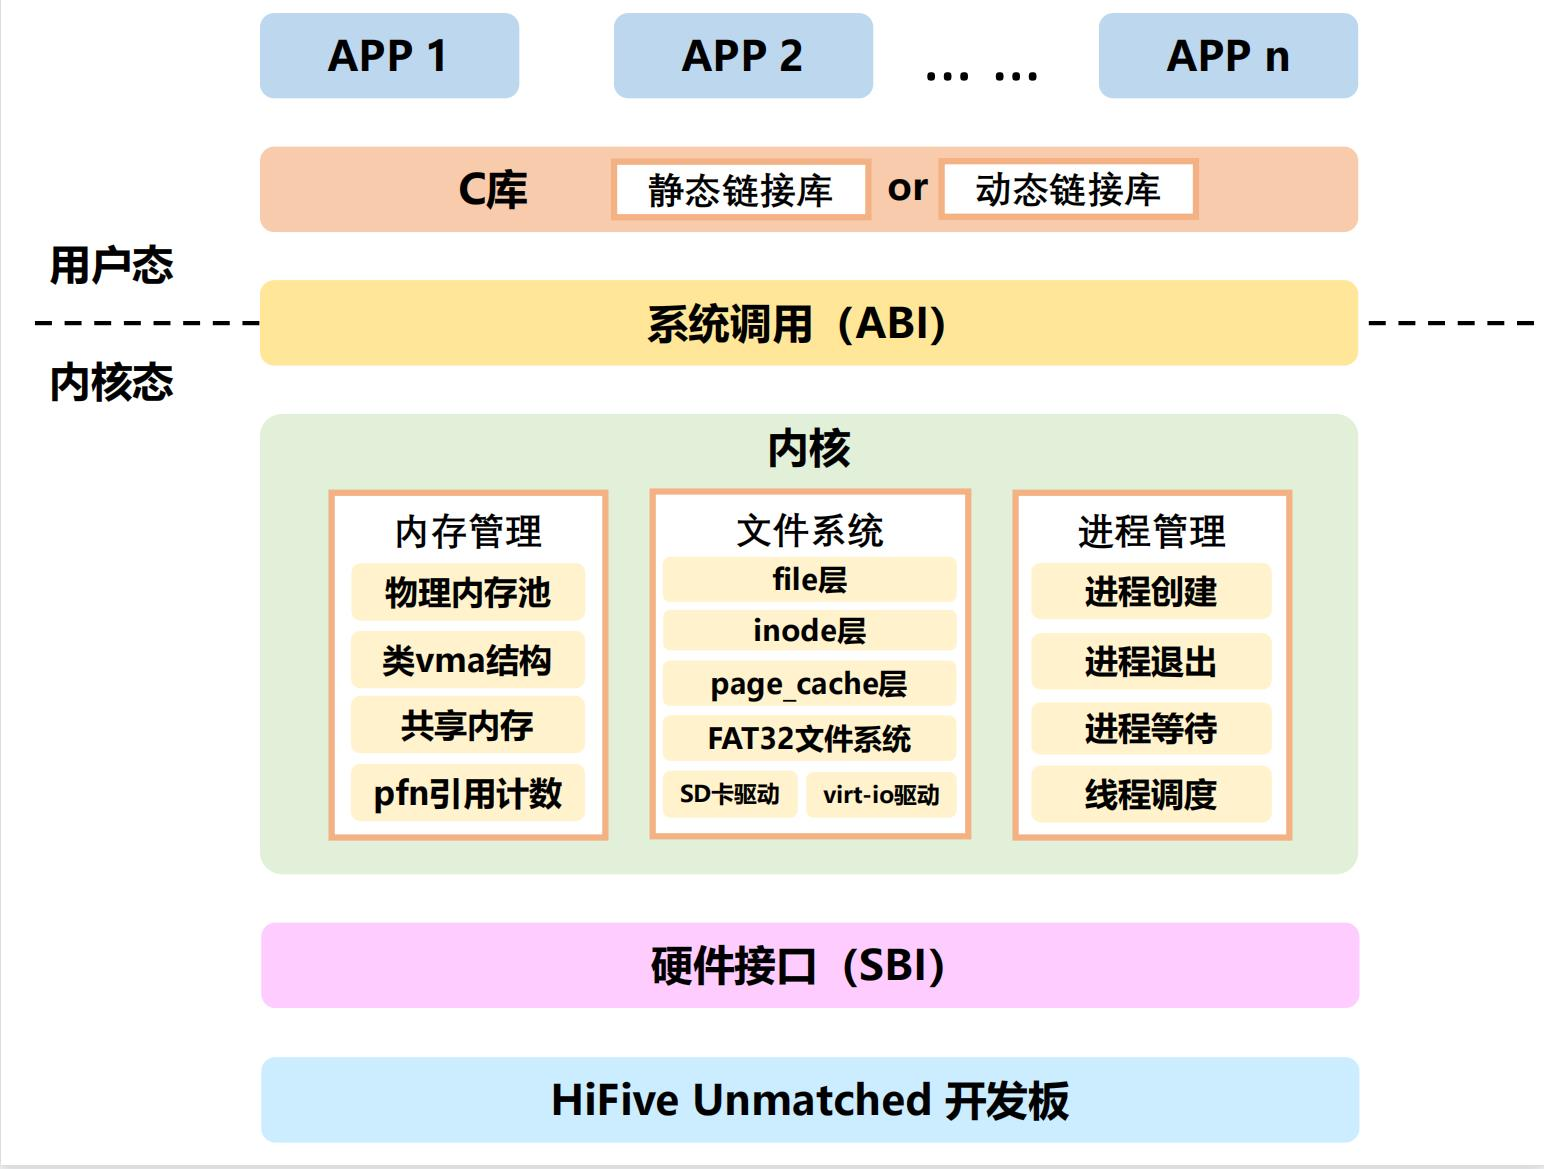
\includegraphics[scale=0.5]{image/img01.jpg}
\end{figure}

ShouChun OS实现框架设计具有\textbf{模块化}的特点,这一点正是对应RISCV架构的特点实现的。
RISCV不同模块组织在一起,成为统一架构,用户可灵活选择模块组合应对不同的应用场景。
对于本项目中较为复杂的操作系统场景而言,同时应用了MachineMode(机器模式)和UserMode(用户模式)。
对应这样的模块组合,操作系统工作的大致流程即:用户应用程序通过库函数(静态或动态链接)发起系统调用请求,
从而实现自身特权级无法完成的操作,内核层作为高特权级在更为安全的情况下完成对应请求。请求的具体实现是通过
硬件接口使用HiFive Unmatched开发板实现的,其中还需要驱动SD卡。
接下来对框架中每一个模块的大致功能实现进行阐述。

\textbf{HiFive Unmatched开发板与SBI(硬件接口)}。HiFive Unmatched开发板具体情况在前文已提及,不作赘述。开发板是具体实现所使用的
硬件实现对于操作系统开发者而言并非擅长之处。为了方便开发者工作,SBI(Supervisor Binary Interface)发挥
了较大的作用。SBI在规定的行业标准下将硬件抽象化,为开发者提供了便捷使用硬件的接口,从而减少了开发者的工作量,又
很好的实现了模块化,使得不同部分的移植更为便捷。ShouChun OS所使用的RISCV运行规范为OpenSBI。

项目工作主要集中在\textbf{内核部分},为了方便项目开发与文档理解,项目将内核部分的设计大致分为三个部分:进程管理、内存管理和文件系统。在成功启动内核后,
三个部分协同工作,完成用户应用程序所要求的功能。其中进程管理主要负责用户进程创建、删除、切换等工作,实现进程部分对用户进程相关请求的相应。内存
管理部分实现内存的分配、释放功能,其中包含有页表相关功能以及堆栈的管理。关于文件系统部分,项目按照比赛要求实现了FAT32格式文件系统,此外由于
比赛要求使用SD卡读取烧写好的测试文件进行测试,ShouChun OS还实现了
SD卡驱动的功能。驱动SD卡功能需要文件系统和SPI共同实现,文件系统模块概念稍后再做详细介绍。SPI
(Serial Peripheral Interface)是一种高速的、全双工的、同步的通信总线,它遵从主-从模式的控制方式,由主设备来控制次设备,为开发者提供
接口来实现外设功能。最终实现了能够对硬盘进行驱动、初始化、读取和写入的功能。FAT32文件系统对于文件实现了抽象化、规范化,使得内核能够更加清晰便捷地管理文件。

\textbf{用户层}各模块相互配合,利用内核所实现的上述工作,使得\textbf{用户应用程序}能够间接实现更高权限的操作,同时又更加具备安全性。这一过程是通过\textbf{系统调用}实现的:
用户应用程序通过\textbf{API层的库函数}来
执行所需功能,库函数可以发起系统调用,通过数据的传递等发起系统调用请求,从而发起中断使操作系统内核执行相关操作并作出响应。

\subsection{内核模块设计}
项目组的工作主要在于内核部分,故接下来针对内核部分的三大模块:进程管理、内存管理、文件系统进行设计展示。
\subsubsection{进程管理}

进程管理部分功能涉及到了进程的创建与回收、进程切换等方面,项目使用统一的
结构体进程控制块(Process Control Block,简称PCB)来进行管理。总的来说
本项目中的进程管理可以使用下图来阐述:

\begin{figure}[H]
  \centering
  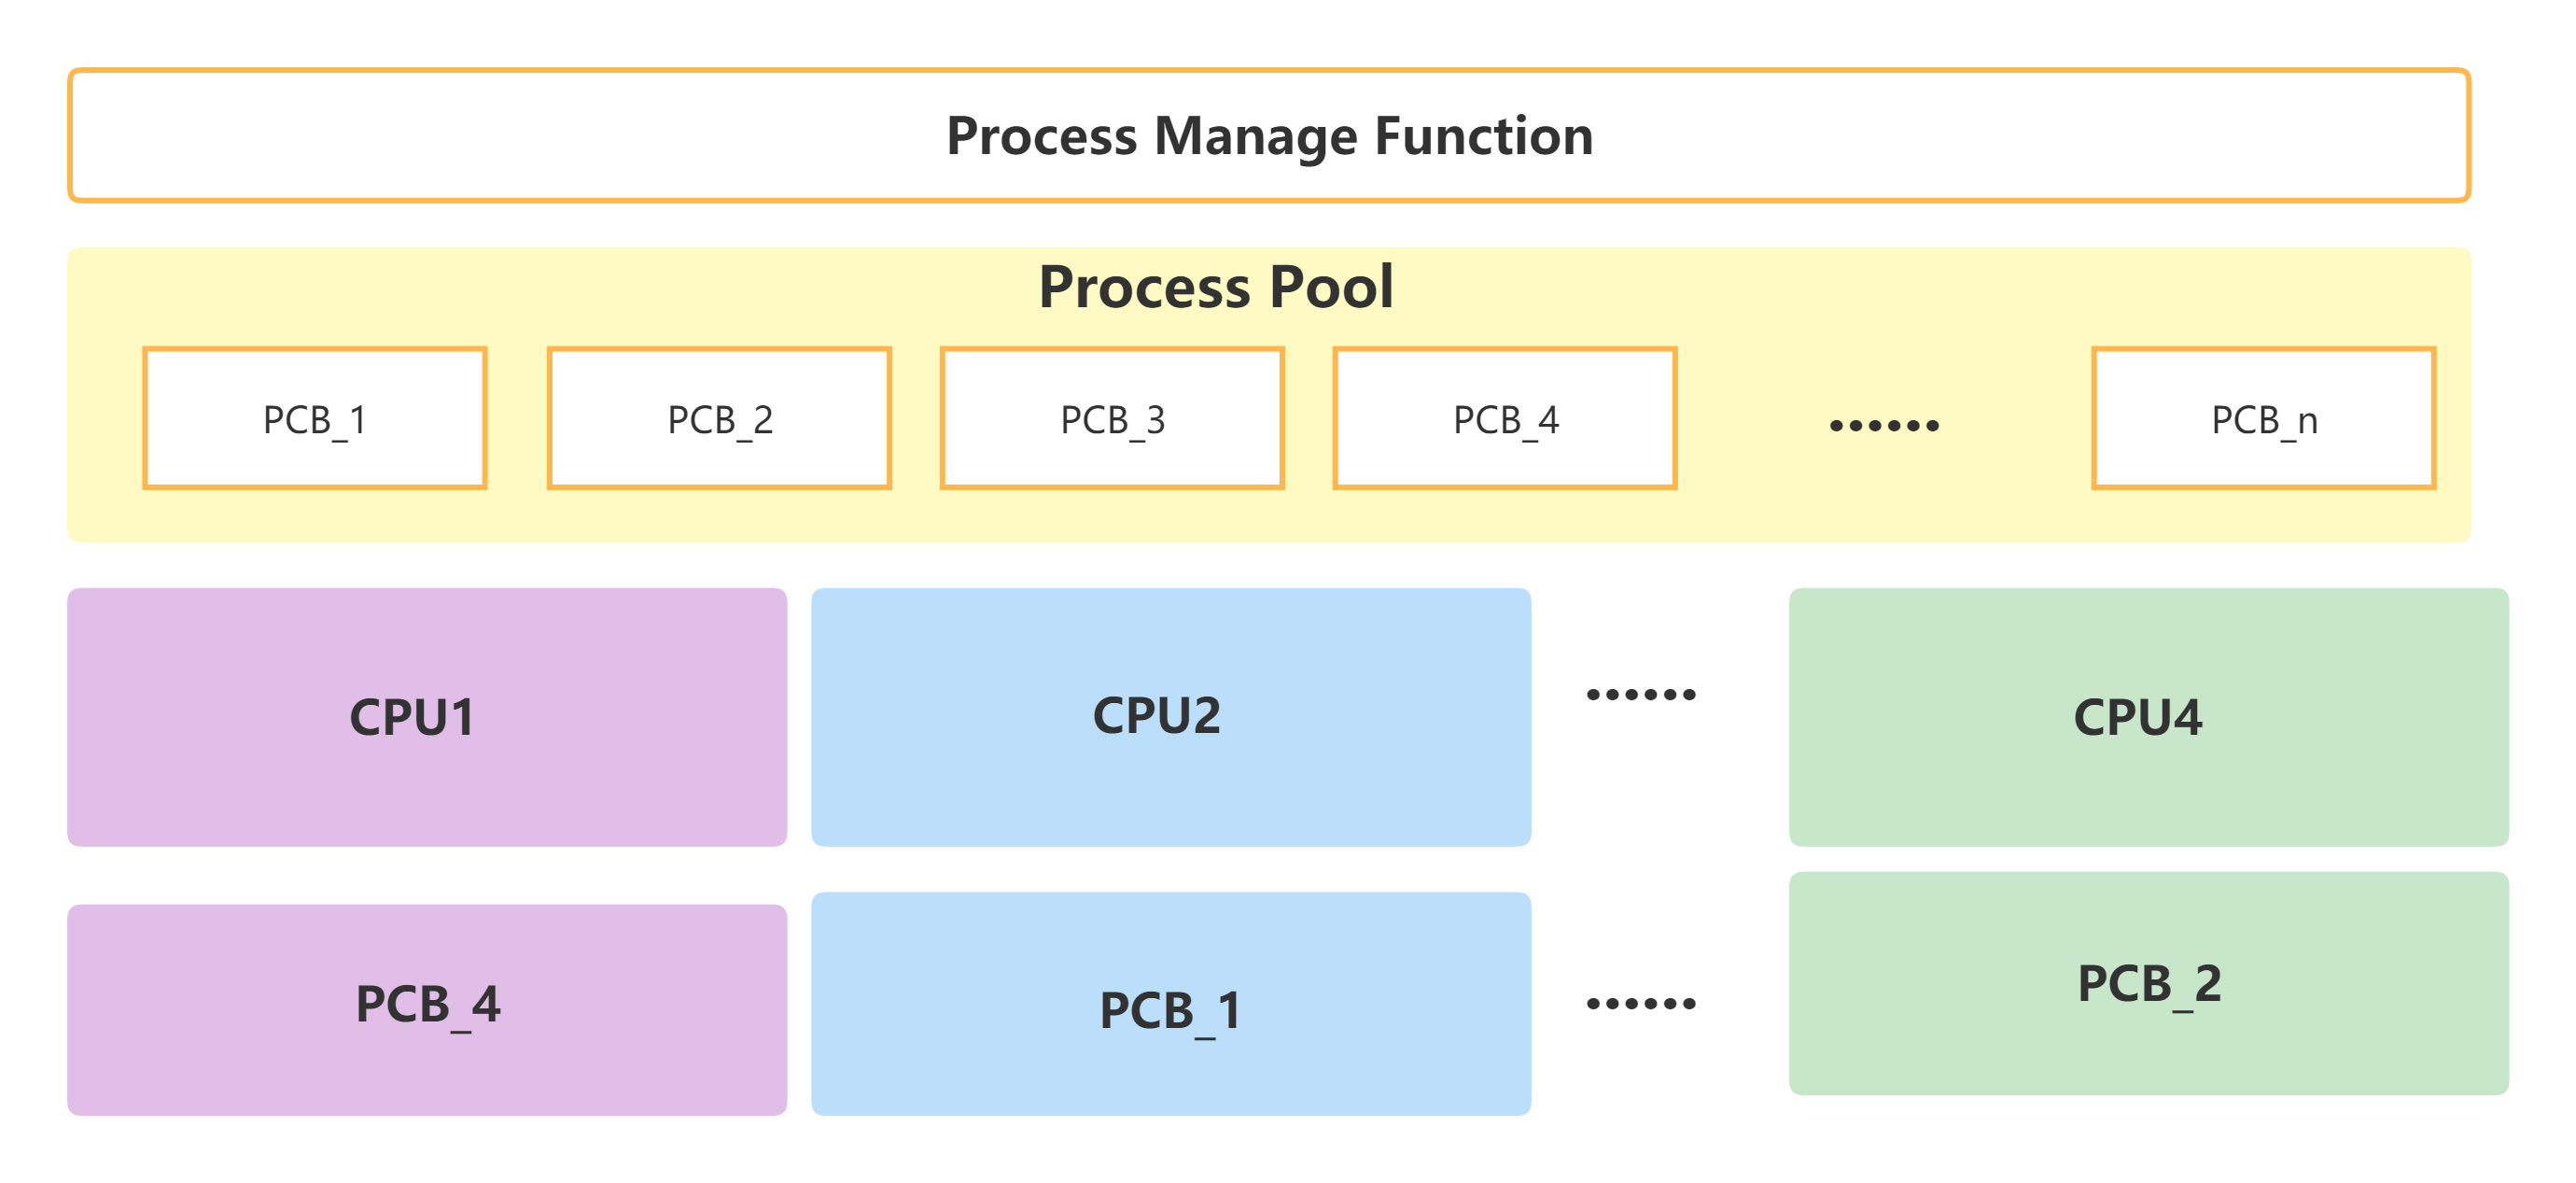
\includegraphics[scale=0.15]{image/design_proc.png}
\end{figure}

自下而上进行解释:
每一个进程都会对应一个进程控制块,用以记录进程基本信息用于管理。
每个核在某一时刻只能运行一个进程,于是核对应着某一个确定的进程控制块。
核所运行的进程来自于进程池。每载入一个进程,就需要放入进程池中等待调度。
进程池中的进程都受进程管理函数的管理。

其中进程管理块中记录了进程运行、管理所需要的信息,包括有进程信息、内存信息、文件
信息等。其中进程信息需要记录的有进程上下文、进程标识符等;内存信息需要记录进程内存大小、
堆栈情况等;文件信息需要记录文件描述符表、路径信息等。其他一些重要信息还包括
时钟、定时器、锁以及实现文件映射所需要的信息等。

核管理器中会记录当前运行进程的进程控制块。进程控制块也可以通过汇编指令来获取
当前核的编号。核管理器和运行进程一一对应。

进程池用于存储所有需要运行的进程。其中的进程会通过进程管理函数进行创建或回收,进程
间的调度切换也是通过这一组管理函数来实现的。

\subsubsection{内存管理}

内存管理部分主要分为内核地址空间、用户地址空间及页表三个部分。其
布局如下图所示。

【内存管理布局示意图】

系统启动、进程管理都在内核地址空间内,每个进程都会分配一个内核栈用以
执行内核态下才能够实现的功能。程序数据存储、动态内存存储等都在用户地址
空间内。内核地址空间和用户地址空间都使用虚拟地址进行实现,虚拟地址和物理
地址之间的转换关系使用页表机制进行实现。ShouChun OS中使用了三级页表进行实现。

\subsubsection{文件系统}

文件系统模块设计图如下:

【文件系统图】

【文字描述】

\section{具体实现}

ShouChun OS主要使用C语言实现,其基于的框架为清华大学陶天骅的\textbf{uCore-SMP}。

\subsection{内核的启动}

内核运行平台为HiFive Unmatched 开发板,其继承了多个内核。其启动过程入下:

【QEMU?】

首先是使用一个python脚本(scripts/kernelld.py)编写内核加载脚本,其中指定了内核
的入口为0x8020000,另外规定了存储布局情况,将用户应用程序的文件名称也写入相应位置【存疑,商议修改】。
在执行完该脚本后,就会得到kernel\_app.ld用于内核的加载。而后会运行scripts/pack.py来
生成链接脚本,该程序用于将用户程序链接打包。

内核加载脚本中指定的入口地址0x80200000即为内核镜像的加载地址,在内核镜像加载完成时即跳转到该入口点处
执行相应内容。我们可以通过汇编文件entry.S来观察这个入口点:

\begin{lstlisting}[title=内核镜像入口,frame=trbl,language={C}]
  .section .text.entry
  .globl _entry
_entry:
  # a0: hartid
  # every core has a boot stack of 4 KB
  la sp, boot_stack
  li t1, 1024*4   # t1 = 4KB
  addi t0, a0, 1  # t0 = hartid + 1
  mul t0, t0, t1  # 4K * (hartid + 1)
  add sp, sp, t0  
  call main

  .section .bss.stack
  .globl boot_stack
  .globl boot_stack_top
boot_stack:
  .space 1024 * 4 * 8
  .globl boot_stack_top
boot_stack_top:
\end{lstlisting}

该汇编文件具体功能即为给当前核分配一个大小为4KB的内核栈空间,
并且将内核栈的地址存储到sp寄存器中,最终调用main()函数启动内核。
在多核系统中,每一个核都会执行该段代码,获取自身的内核栈空间,使得
不同核运行在不同的位置处(这一位置是与内核编号相关的),互不影响,并行工作。

在跳转到main函数后,会进行操作系统的初始化等操作。此时尚未成功在
FU740上成功启动多核。项目具体的实现方法为:在完成初始化操作后,\textbf{由当前
启动的核来启动其他核},该用于启动其他核的核为第一次启动。启动是通过\textbf{SBI接口}来实现
的,需要传参所需启动核的编号。以下为具体启动核的SBI接口函数:

\begin{lstlisting}[title=内核镜像入口,frame=trbl,language={C}]
void start_hart(uint64 hartid,uint64 start_addr, uint64 a1) {
    a_sbi_ecall(0x48534D, 0, hartid, start_addr, a1, 0, 0, 0);
}
\end{lstlisting}

启动内核使用的main函数大致如下(省略信息展示与初始化部分)。

\begin{lstlisting}[title=内核启动的main函数,frame=trbl,language={C}]
  void main(uint64 hartid, uint64 a1) {
    if (first_hart) {
      // 计算机信息展示...
      // 初始化工作...
        if (hartid >= NCPU){
            panic("unexpected hartid");
        }
        int CPU_START=1;    // core 0 is not usable
        for (int i = CPU_START; i < NCPU; i++) {
            if (i != hartid && i!=0) // not this hart
            {
                printf("[ucore] start hart %d\n", i);
                start_hart(i, (uint64)_entry, 0);
                while (booted[i] == 0){
                    // wait
                }
            }
        }
        wait_all_boot();
    } else {
        hart_bootcamp(hartid, a1);
    }
    while (!all_started) {
        ; // wait until all hard started
    }
    // 内核运行
}
  \end{lstlisting}

可以看到,当前启动核为\textbf{第一次启动}时,就会用于遍历启动其他所有核;当判断到当前核并非初次
启动时,就说明无需帮忙其他核,初始化与其他核的独立部分即可。等待所有核启动后,各个核
再进入运行状态。\textbf{需要注意的是},FU740具有四个大核以及一个小核,小核并不能通过SBI
启动,所以启动时内核编号需要从1开始。

\subsection{elf loader:可执行程序加载}

elf loader用于将ELF格式的可执行程序加载到内存中,在该系统中支持静态链接和动态链接两种程序的加载。

其简化的流程图如下:

【流程图】

对于静态链接程序,将可执行程序按照ELF头中的信息加载到内存中即可。

对于动态链接程序,除了需要加载可执行程序外,还需要将解释器加载到内存中。解释器的作用是根据系统加载器提供的AUXV信息,通过mmap系统调用,加载动态链接程序依赖的所有动态链接库,并且对动态链接库进行重定向,最终跳转到动态链接程序入口,此时解释器的工作完成。

AUXV中的信息主要包括以下几个部分,这些信息对于解释器来说是必要的:

\begin{lstlisting}[title=AUXV信息,frame=trbl,language={C}]
  #define AT_PHDR         3               /* Program headers for program */
  #define AT_PHENT        4               /* Size of program header entry */
  #define AT_PHNUM        5               /* Number of program headers */
  #define AT_PAGESZ       6               /* System page size */
  #define AT_BASE         7               /* Base address of interpreter */
  #define AT_ENTRY        9               /* Entry point of program */
  \end{lstlisting}

其中AT\_PHDR、AT\_PHENT、AT\_PHNUM、AT\_ENTRY用于给解释器提供可执行程序的各种信息,
解释器会解析可执行程序的ELF头,找找到依赖的动态链接库文件并加载到内存中。AT\_BASE是解释器的加载地址,用于解释器获取自身信息并进行重定向工作。AT\_PAGESZ是系统页面大小,在该系统中该数值为常数0x1000。

在系统加载器加载完毕后,会将argv、envp、auxv参数存放在用户态栈中,提供给应用程序与C库使用,栈结构如下:

【栈结构】
  

\subsection{中断异常机制}

中断机制在系统中起着\textbf{通信网络}的作用,可以协调系统对各种外部事件的响应和处理。
中断是CPU 对系统发生的某个事件作出的一种反应。引起中断的事件称为\textbf{中断源}。
中断源向CPU 提出处理的请求称为\textbf{中断请求}。发生中断时被打断程序的暂停点称为\textbf{断点}。
CPU暂停现行程序而转为响应中断请求的过程称为\textbf{中断响应}。处理中断源的程序称为\textbf{中断处理程序}。
CPU执行有关的中断处理程序称为\textbf{中断处理}。

\subsubsection{中断处理}

中断处理所使用的到结构体为\textbf{trapframe}:

\begin{lstlisting}[title=trapframe结构体,frame=trbl,language={C}]
  struct trapframe {
    /*   0 */ uint64 kernel_satp;   // kernel page table
    /*   8 */ uint64 kernel_sp;     // top of process's kernel stack
    /*  16 */ uint64 kernel_trap;   // usertrap()
    /*  24 */ uint64 epc;           // saved user program counter
    /*  32 */ uint64 kernel_hartid; // saved kernel tp
    // ...... 寄存器
    /* 280 */ uint64 t6;
};
  \end{lstlisting}

trapframe中主要内容为\textbf{发生中断异常时的现场情况},其中kernel\_satp给出了内核页表的地址;
kernel\_sp指向了进程内核栈的顶部;kernel\_trap指向usertrap函数,用于在用户状态下发生
中断时跳转到处理函数。

用户状态下中断处理流程图如下:

【作图】
【存疑】

中断的处理需要使用的函数为usertrap,在trap.c文件中。每次出现中断或者异常时,都需要跳转到中断入口处,
执行trampoline.S汇编代码的内容,即先保存当前用户程序的现场到trapframe当中,最后取出kernel\_trap中
所存储的usertrap函数的地址,最终跳转到该函数处进行中断的处理。在usertrap中,会首先将kernelvec的地址写入
stvec中,作为中断处理的基址,此时的中断为需要\textbf{升高权限为内核态}所处理的中断了。usertrap处理
中断时,分为了中断和异常两种情况。其中中断包括有计时器发起的中断和外部设备发起的中断;异常包含了指令异常和页
加载异常等等,本项目中心工作所集中的系统调用便包含在异常当中,具体处理异常的代码如下:

\begin{lstlisting}[title=系统调用异常,frame=trbl,language={C}]
  case UserEnvCall:   // 8
  if (p->killed)
      exit(-1);
  trapframe->epc += 4;
  intr_on();
  syscall();
  break;
  \end{lstlisting}

在用户态发起系统调用异常后,会使用\textbf{syscall函数}作为接口,读取trapframe中所记录的系统调用号
以及参数,从而在syscall函数中找到对应的中断处理函数。将参数传给相应的中断处理函数并执行结束后,
将返回值存储在trapframe的a0中,最终返回时会通过存储的地址返回调用位置,恢复触发中断前的现场。
本项目中内核态下的中断主要是\textbf{时钟中断与外部中断},其他情况下的中断与异常均作为意外情况,使用panic
退出程序。

\subsection{进程管理}

\subsubsection{相关系统调用}

进程管理部分相关的系统调用如下:

\begin{lstlisting}[title=进程管理系统调用,frame=trbl,language={C}]
  #define SYS_clone 220
  #define SYS_execve 221
  #define SYS_wait4 260
  #define SYS_exit 93
  #define SYS_getppid 173
  #define SYS_getpid 172
\end{lstlisting}

\subsubsection{核心结构体proc}

进程管理的实现主要是通过核心的\textbf{结构体proc}实现的。进程管理的核心结构体为proc,其定义如下:

\begin{lstlisting}[title=proc结构体,frame=trbl,language={C}]
  struct proc {
    struct spinlock lock;

    // PUBLIC: p->lock must be held when using these:
    enum procstate state;  // Process state
    int pid;               // Process ID
    int killed;            // If non-zero, have been killed
    pagetable_t pagetable; // User page table
    void *waiting_target;  // used by sleep and wakeup, a pointer of anything
    uint64 exit_code;      // Exit status to be returned to parent's wait

    // proc_tree_lock must be held when using this:
    struct proc *parent; // Parent process

    // PRIVATE: these are private to the process, so p->lock need not be held.
    uint64 ustack_bottom;        // Virtual address of user stack
    uint64 kstack;               // Virtual address of kernel stack
    struct trapframe *trapframe; // data page for trampoline.S, physical address
    struct context context;      // swtch() here to run process
    uint64 total_size;           // total memory used by this process
    uint64 heap_start;           // start of heap
    uint64 heap_sz;
    uint64 stride;
    uint64 priority;
    uint64 user_time;           // us, user only
    uint64 kernel_time;         // us, kernel only
    uint64 last_start_time;     // us
    struct file *files[FD_MAX]; // Opened files
    struct inode *cwd;          // Current directory
    struct shared_mem * shmem[MAX_PROC_SHARED_MEM_INSTANCE];
    void * shmem_map_start[MAX_PROC_SHARED_MEM_INSTANCE];
    void* next_shmem_addr;
    struct mapping maps[MAX_MAPPING];
    char name[PROC_NAME_MAX]; // Process name (debugging)
};
  \end{lstlisting}

进程管理相关的操作大部分都是基于此结构体进行实现的。proc结构体
的成员从\textbf{性质}层面来看,大致可以分为\textbf{公开资源和私有资源}两个部分,可用以实现
多进程安全并行;从\textbf{功能}方面来看,proc成员分为四类:进程的基本信息、
进程的内存信息、进程文件信息和其他信息。

\textbf{进程的基本信息}包括了进程编号、进程上下文、父进程等。其中state为进程的状态,
包括有UNUSED、USED、SLEEPING、RUNNABLE、RUNNING、ZOMBIE六种情况,利用
这几种状态就可以实现进程的调度和回收等功能;pid为进程编号,是进程
重要的成员属性,大多进程管理相关操作都基于此实现;parent记录了父进程,用于
进程之间关系的管理;context记录了进程的上下文,用于进程的切换;trapframe陷阱帧
用于异常中断机制的运行现场恢复;exit\_code用于
在子进程退出时将退出状态码放回给父进程。

\textbf{进程的内存信息}包括进程占用的地址空间、堆以及共享内存信息。ustack\_bottom、kstack、
heap\_start分别记录了用户栈、内核栈、堆的地址,这里的地址指虚拟地址;
maps用来记录文件载入后映射的情况;pagetable记录了当前进程所使用
的页表,从而进行虚拟地址和物理地址之间的转换。

\textbf{进程的文件信息}包括了文件描述符数组和当前位于目录。files记录了所有已经打开的文件描述符;cwd可
获取当前所处的目录。

\textbf{其他信息}包含了运行时间、信号、优先级、调度权等,辅助进行进程的管理。结构体中的成员lock用于实现进程锁,从而达成多进程并行执行而互不影响。
进程锁的使用对进程公开资源的修改来说十分重要。

\subsubsection{进程管理方法}

一个核可以同时运行多个进程,内核使用了\textbf{进程池}来对进程进行管理。结合proc结构、pool进程池和其他一些重要辅助信息,
可以完成进程的创建、销毁、调度和调度等功能。

(1)\textbf{进程的创建与销毁}:在创建进程时,会在进程池中找到一个可用的进程号(pid),进行初始化。proc唯一对应一个
进程,创建时将根据程序内容构建处用户地址空间并分配物理空间。当进程退出时,需要对进程进行销毁,释放其占用的进程池
中的可用pid,并重新初始化结构体。

(2)\textbf{进程调度方法}:进程的调度使用 \textbf{Stride算法}。该种算法为不同的进程分配了不同的优先级,每个进程得到的时间资源
预期优先级成正比。以下是调度所使用的代码(只列出了调度相关的核心部分):

\begin{lstlisting}[title=进程调度方法,frame=trbl,language={C}]
void scheduler(void)
{
    // ...
    for (;;){
        uint64 min_stride = ~0ULL;
        struct proc *next_proc = NULL;
        int any_proc = FALSE;

        for (struct proc *p = pool; p < &pool[NPROC]; p++){
            if (!p->state == UNUSED){
                any_proc = TRUE;
                // debugcore("state=%d", p->state);
            }
            if (p->state == RUNNABLE && !p->lock.locked){
                if (p->stride < min_stride){
                  //找到stride最小的进程
                    min_stride = p->stride;
                    next_proc = p;
                }
            }
        }
      // ...
        if (next_proc != NULL)
        {
            //...
            //计算步长pass并更新stride
            uint64 pass = BIGSTRIDE / (next_proc->priority);
            next_proc->stride += pass;
            //进行进程的切换
            swtch(&mycpu()->context, &next_proc->context);
            //...
        }
        else{
          //...
        }
       //...
    }
}
  \end{lstlisting}

  \textbf{算法基本思想}为:

1.为处于\textbf{RUNNABLE状态}的进程设置优先级,表示进程当前的调度权。并定义pass值,表示
相应进程在调度后,stride需要累加的值。

2.在每次需要调度时,从当前RUNNABLE状态的进程中选择stride\textbf{最小}的进程进行调度。

3.获得调度的进程,将其stride加上对应的步长pass(pass值只与\textbf{进程的优先权}有关)。

4.在一段固定时间后,回到步骤2,重新进行调度,运行当前进程池中stride最小(非0)的进程。

其中,调度进程时的\textbf{切换过程}为:首先保存当前进程的上下文(context),而后再通过所需调度进程的上下文恢复所需调度进程
的现场,从而实现调度。具体内容在汇编文件switch.S中。

(3)\textbf{创建子进程}:创建子进程实际也是实现fork的方法,在执行fork操作时,当前进程,即父进程,会构造一个
与自己完全相同的用户空间,并分配对应的空间、pid以及内核栈,新得到的进程即为子进程。

【要不这里再加一下重点的进程系统调用实现】

\subsection{内存管理}

\subsubsection{相关系统调用}

\begin{lstlisting}[title=内存管理系统调用,frame=trbl,language={C}]
#define SYS_brk 214
#define SYS_munmap 215
#define SYS_mmap 222
\end{lstlisting}

\subsubsection{内核态内存管理}

在系统启动后,首先处于没有开启分页的状态,访问的地址全部是物理地址,因此首先需要构建\textbf{内核态页表},
该任务由kvminit函数完成。在内核态中,几乎保持所有映射均为\textbf{虚拟地址=物理地址},便于管理内存。

内核态内存布局如下:

【作图】

其中\textbf{I/O空间部分的映射用于与外设交互}。其中PLIC为中断控制器地址,用于控制中断开关,
获取中断信息。VIRT I/O为qemu的mmio地址,用于在qemu中读取磁盘文件。
SPI地址为fu740的SPI端口地址,用于读写SD卡。

从0x80200000开始为\textbf{内核镜像},其中代码段映射访问权限为RX,数据段映射访问权限为RW。这部分内容由上一启动阶段的U-Boot加载到内存中。

从内核镜像末尾到0x88000000均作为\textbf{物理内存池},用于给内核中的部分动态数据结构、所有用户态进程分配内存。

另外,评测机将SD卡镜像加载到了0x90000000位置,我们也对此地址范围进行了映射,用于\textbf{读写SD卡内容}。

除此之外,在虚拟地址为0x3FFFFFF000的位置还映射了trampoline,
在用户态内存中的相同虚拟地址同样也映射了trampoline,trampoline是一小段代码,
这段代码用于\textbf{衔接用户态和内核态之间的切换},在由用户态进入到内核态时,
需要保存上下文,构造trapframe,并跳转到异常处理函数,在由内核态退出到用户态时,
需要根据trapframe还原上下文。

(1)物理内存池

物理内存池结构如下:

【作图】

空闲页面依靠\textbf{单向链表}连接,每个空闲页面的头部是一个list\_entry,指向下一个空闲页面。

每次需要分配页面时,则从链表头部摘下一个节点,当页面释放时,则重新加入空闲页面链表。

(2)pfn引用计数

由于该系统支持文件mmap映射,因此会存在多个进程的虚拟地址映射到相同物理页的情况,
因此为了正确实现物理页面资源的管理,
需要记录\textbf{物理页面引用计数},记录的数据结构如下:

\begin{lstlisting}[title=页面引用计数,frame=trbl,language={C}]
  uint8 pfn_ref[(PHYSTOP - KERNBASE) >> PGSHIFT];
\end{lstlisting}

每个页面分配时,在pfn\_ref中将对应位置置为1,
当页面被再次引用时,则引用计数加1,当页面被释放时,
引用计数减1,当引用计数变为0时,则该页面变为空闲状态,放入空闲链表中。

(3)多进程内核栈分配

在多进程运行过程中,内核地址空间被划分为了多个内核栈空间,
对应不同的用户进程:

【无Guard Page?】

【内核地址空间示意图】

每个进程对应着自己唯一的内核栈。当新建一个进程时,都需要为其分配内核栈空间。以下是新建进程时给进程分配内核栈的代码:

\begin{lstlisting}[title=分配内核栈空间,frame=trbl,language={C}]
struct proc *alloc_proc(void) {
    // ......
    memset(&p->context, 0, sizeof(p->context));
    p->kstack = (uint64)kstack[p - pool];
    memset((void *)p->kstack, 0, KSTACK_SIZE);

    p->context.ra = (uint64)forkret; // used in swtch()
    p->context.sp = p->kstack + KSTACK_SIZE;
    // ......
}
\end{lstlisting}

可以看到,\textbf{内核栈空间的分配方法}为:从划分好的内核栈分配中选取对应进程池位置的
内核栈。也就是说,每个进程对应着进程池中唯一的一个proc指针,每一个proc都对应着固定
的内核栈地址。\textbf{内核栈设置方法}为定义NPROC×KSTACK\_SIZE大小的二位字符数组,
即最多可同时给NPROC(256)个进程分配内核栈,且内核栈大小为KSTACK\_SIZE(8192),【由于分配的
内核栈大小足够大,故未使用guardpage分隔内核栈】

\subsubsection{用户地址空间}

用户态所有数据所占内存全部由内核中的\textbf{物理内存池}提供。

用户态内存布局如下:

【用户地址空间示意图】

本项目使用了SV39虚拟内存,支持高达256GB的用户内存空间。
由ELF装载地址(默认为0x1000)到heap\_start之间的地址空间用于装载ELF可执行程序的各个段。
由heap\_start到heap\_start + heap\_sz之间的地址空间是堆空间,其作为动态分配的空间从堆栈底部向高地址增长。
栈空间从0xC0000000向低地址增长,目前设定栈大小为25个页面大小。在堆空间和栈空间之间的是mmap区域,
用于动态申请内存或映射文件,向低地址方向增长。用户空间的顶部为trampoline,将虚地址和实地址对应了起来,可用于在多进程并行时切换进程。
Trampoline下存储着4KB大小的TrapFrame用于中断异常处理。

其中mmap区域内存映射信息使用了\textbf{mapping结构}进行记录:

\begin{lstlisting}[title=mapping结构,frame=trbl,language={C}]
  struct mapping {
    uint64 va; // must be PGSIZE aligned
    uint npages;
    bool shared;
};
  \end{lstlisting}

每个进程都有一个mapping结构体数组,作用类似于Linux中的vma,
用于存放mmap映射信息,其中shared记录用于判断在进程克隆时该映射是否与子进程共享。

\subsubsection{页表机制}

虚拟地址的管理使用了\textbf{页表机制},进程在访问到记录好的页表的物理地址后,可以通过页表
转换找到虚拟地址所对应的物理地址。

(1)\textbf{页表机制的使能}。虚拟地址和物理地址之间的映射关系记录在了页表当中,可以通过mmap函数和munmap函数进行
这种关系的管理。本系统中,所有进程内核态下虚拟地址与物理地址之间的对应关系都是相同的。
进程在一开始启动时就会初始化内核空间的页表,内核空间的映射关系为
固定的直接映射,使用kvmmap函数将其记录到了内核页表当中。注意在这一初始化内核页表的过程中不刷新
块表和开启页表机制,在进程加载好内核页表后,才可以使能页表机制。

(2)\textbf{三级页表机制}。Sv39页表机制是具有三级页表的,虚拟地址将分为五个部分(下图为示意图):
39-63位使用0进行填充,30-38位为页目录项,21-29位为一级页表项,12-20位为二级页表项【存疑】,
0-11位为业内偏移地址。

【虚拟地址分块示意图】

其寻址方法流程如图所示,首先访问记录好的进程对应页表位置,取30-38位偏移找到对应页表的
物理位置,而后取21-29位在页表内偏移找到对应页表项所记录的二级页表的物理地址,而后访问二级页表
根据12-20位找到对应物理页的位置,最终根据页内偏移即可访问正确的地址。该部分对应了函数
walk(位于virtual.c文件当中)。

【寻址示意图】

\subsubsection{系统调用实现}

该部分系统调用的实现主要体现在brk和mmap、munmap。

(1)brk的实现

brk系统调用用于调整堆内存大小,首先将新栈顶指针与堆起始地址比较,防止新地址低于堆起始地址。

\begin{lstlisting}[title=检查brk参数,frame=trbl,language={C}]
if ((uint64)addr < p->heap_start) {
    infof("sys_brk: addr is below heap start");
    return -1;
}
\end{lstlisting}

然后根据新栈顶指针的位置,决定申请内存/释放内存。【TODO】

\begin{lstlisting}[title=brk实现,frame=trbl,language={C}]
uint64 old_pos = p->heap_start + p->heap_sz;
uint64 new_pos = (uint64)addr;
if (new_pos > old_pos) {
    // allocate memory
    new_pos = uvmalloc(p->pagetable, old_pos, new_pos);
} else {
    // deallocate memory
    new_pos = uvmdealloc(p->pagetable, old_pos, new_pos);
}
\end{lstlisting}

(2)mmap和munmap的实现



\textbf{mmap用于申请内存、映射文件、实现共享内存},其内部实现较为复杂,
目前支持MAP\_SHARED、MAP\_PRIVATE、MAP\_FIXED、MAP\_ANONYMOUS、MAP\_FILE 类型的请求,
简化的流程图如下:

【作图】

对于文件映射类请求,由于在文件系统的设计中实现了page cache层,因此可以很容易的获得文件对应的物理页面,
并将其映射到进程地址空间中。当某进程需要使用磁盘上的某一部分内容时,需要先在内核空间中为其分配一定大小的空间作为缓存
,调用mmap函数来建立该部分内容到虚拟内存的映射,并使用页表记录这一关系。
当有其他进程要求访问该部分内存时,可以通过sys\_mmap调用来
直接使用这段已经加载入内核空间的内容,同时更新该段内容的使用情况。当进程结束访问后,就会
调用sys\_munmap函数来释放其对该部分内存的引用,当其引用数清零时,即可删除这一映射关系,释放对应
部分的内存。

【文件读写图】

文件映射除了可以用于加快文件读写速度,还可以用于实现\textbf{共享内存},
当两个进程以MAP\_SHARED方式映射了同一个文件的同一位置后,
则该page\_cache物理页映射到了两个进程地址空间中,即可实现共享内存。

【共享内存图】

对于内存申请类请求,实现的难点主要在于对MAP\_FIXED的处理,根据MAP\_FIXED标志的说明,
对于新申请的内存区间与已有内存区间存在交集时,需要将overlap的区间释放掉,
因此就涉及到对\textbf{mapping数据结构的拆分与合并}问题,因此新加入了以下三个函数用于解决该问题。

\begin{lstlisting}[title=mapping数据结构的拆分与合并,frame=trbl,language={C}]
  uint64 old_pos = p->heap_start + p->heap_sz;
  uint64 new_pos = (uint64)addr;
  if (new_pos > old_pos) {
      // allocate memory
      new_pos = uvmalloc(p->pagetable, old_pos, new_pos);
  } else {
      // deallocate memory
      new_pos = uvmdealloc(p->pagetable, old_pos, new_pos);
  }
  \end{lstlisting}


在处理MAP\_FIXED请求时,首先需要对overlap的区间调用mapping\_try\_remove\_page和uvmunmap进行释放,
若成功释放掉了overlap区间,则继续后续处理,否则映射失败。

在处理普通的\textbf{内存申请请求}时,若给定address不是NULL,则将给定address作为hint,
基于此地址向高地址搜索空闲区间,否则则按照mmap增长方向,由高地址向低地址搜索空闲区间。

munmap实现较为简单,只需将参数按照页面大小对齐,
然后对给定区间调用mapping\_try\_remove\_page和uvmunmap释放内存。

\subsection{文件系统}

在系统中,对fat32文件系统进行了多层封装,并且对应用程序提供了类Unix的文件系统操作接口。

其层次结构如下:

【层次结构图】

\subsubsection{相关系统调用}

系统中实现的文件系统相关syscall如下,
相关函数位于syscall/syscall\_impl.c中。
除比赛要求的syscall外,为了支持libc-test的多个测试点,
还对SYS\_lseek、SYS\_readv、SYS\_writev、SYS\_fstatat提供了支持。

\begin{lstlisting}[title=文件系统相关先系统调用,frame=trbl,language={C}]
  #define SYS_getcwd 17
  #define SYS_mknod 33
  #define SYS_mkdirat 34
  #define SYS_linkat 37
  #define SYS_unlinkat 35
  #define SYS_chdir 49
  #define SYS_openat 56
  #define SYS_close 57
  #define SYS_pipe2 59
  #define SYS_getdents64 61
  #define SYS_lseek 62
  #define SYS_read 63
  #define SYS_write 64
  #define SYS_readv 65
  #define SYS_writev 66
  #define SYS_fstatat 79
  #define SYS_fstat 80
  \end{lstlisting}

  文件系统相关syscall的主要作用是接收用户传入的参数,
  将字符串等参数从进程的地址空间复制到内核空间,
  便于后续的层进一步处理,然后对参数进行合法性检验,
  过滤掉一些不合法、不支持的系统调用请求。
  在这一层中还需要将用户传入的fd转换成struct file*,
  然后将请求发送给下一层:file层。【TODO】
  
  【file\_syscall.png】

\subsubsection{file层}

file层操作的对象为file结构体,每个file结构体是进程独有的,因此不需要使用锁防止对该数据结构的并行操作,
主要工作是维护file结构体内的各个属性,包括引用计数、读写权限等信息,
并取出内部的struct inode指针,将请求转发给inode层。

\subsubsection{inode层}

inode层负责管理磁盘上的文件、目录,每一个inode结构体都是对普通文件、设备文件或目录的抽象,
由于inode是对某个文件/目录的抽象,而不与具体进程绑定,inode可以被多个进程共享,
因此存在多线程冲突问题,需要使用锁来避免对inode数据结构的并行操作。
大部分inode层的函数要求获得inode的锁以后才可以使用。

在目前的设计中,由于仅需要支持FAT32文件系统,因此inode结构体和fatfs中的文件、目录数据结构绑定,
更好的设计是在此处插入虚拟文件系统层(vfs),使得inode与fatfs解绑,从而降低耦合性,
便于支持多种文件系统。

(1)设备文件

已支持的设备文件包括:console、cpu、mem、proc、null、zero

设备文件的存储格式如下:(可以举例子作图)

{4字节:'devx'}{4字节:major}{4字节:minor}

从文件中读取出上述信息后,根据major号调用相应handler函数进行处理。

(2)符号链接

目前仅支持普通文件/设备文件类型的符号链接,不支持目录的符号链接,主要用于链接libc库的动态链接库文件。

符号链接文件的存储格式如下:(可以举例子作图)

{4字节:'slnk'}{n-4字节:链接文件绝对路径}

从文件中读取出上述信息后,根据链接文件的绝对路径打开连接的文件。

(3)普通文件

若判断类型为文件,但并不是设备文件、符号链接,则认定该文件为普通文件,通过fatfs接口的f\_open打开该文件。

(4)目录

若判断类型为目录,则通过fatfs接口的f\_opendir函数打开该目录。

\subsubsection{page\_cache层}

为了提高I/O速度,同时为了支持mmap,因此在inode下层加入page\_cache层,
在该系统中page\_cache的设计思想与Linux类似,但是具体实现有所不同。

在 Linux 2.4 版本的内核之前,page cache 与 buffer cache 是完全分离的。
但是,块设备大多是磁盘,磁盘上的数据大多通过文件系统来组织,
这种设计使得读写文件需要经历五个步骤(如下图):将文件数据块加载入页缓存中,
页缓存中文件内容读入内存,修改内存对应部分,将修改后的内容写入到页缓存,
页缓存写回磁盘。这就导致很多数据被缓存了两次,浪费内存。

为了提高效率,在该系统的设计中剔除了buffer cache,
仅使用page cache,从而减少了数据的缓冲次数。

由于磁盘I/O对系统性能影响较大,因此在page cache的设计中选择了cache命中率较高的LRU淘汰算法,
而没有选择random淘汰算法。

【作图】

由于大多数操作可以由处在内存中的page cache满足,而不需要进行磁盘I/O操作,
因此在普通读写中可通过page cache提高I/O速度。

【作图】

为了再次减少内存拷贝的次数,可以使用mmap将page cache的物理页面直接映射到应用程序的地址空间内,
从而实现更加高效的文件I/O操作。

【作图】

\subsubsection{FAT32文件系统驱动}

FAT32文件系统驱动采用的是嵌入式系统常用的FatFs文件系统驱动:http://elm-chan.org/
fsw/ff/00index\_e.html

FatFs提供了完备的FAT系列文件系统操作接口,支持FAT16、FAT32、exFAT。
但是该文件系统驱动提供的接口接近Windows驱动的接口,
因此在该系统中对该驱动进行了多层包装,最终对应用程序提供类Unix的文件系统操作接口。

\subsubsection{sd卡驱动}

sd卡驱动移植自fu540 bootloader:https://github.com/sifive/freedom-u540-c000-bootloader,支持通过SPI以忙等待的方式与SD卡通信,暂不支持DMA方式读写。

SD卡通信协议参考了SD Specifications的物理层部分。

SPI地址参考自fu740手册。

代码位置:os/driver/sd.c

(1)sd卡驱动初始化

首先将SPI内存区域映射进内核地址空间,然后通过SPI给SD卡发送启动命令,最后重新设置分频,提高I/O性能。

初始化部分代码如下:

\begin{lstlisting}[title=sd卡驱动初始化,frame=trbl,language={C}]
  int sd_init(spi_ctrl* spi, unsigned int input_clk_khz, int skip_sd_init_commands)
  {
    // Skip SD initialization commands if already done earlier and only set the
    // clock divider for data transfer.
    if (!skip_sd_init_commands) {
      sd_poweron(spi, input_clk_khz);
      if (sd_cmd0(spi)) return SD_INIT_ERROR_CMD0;
      if (sd_cmd8(spi)) return SD_INIT_ERROR_CMD8;
      if (sd_acmd41(spi)) return SD_INIT_ERROR_ACMD41;
      if (sd_cmd58(spi)) return SD_INIT_ERROR_CMD58;
      if (sd_cmd16(spi)) return SD_INIT_ERROR_CMD16;
    }
    // Increase clock frequency after initialization for higher performance.
    spi->sckdiv = spi_min_clk_divisor(input_clk_khz, SD_POST_INIT_CLK_KHZ);
    return 0;
  }
  \end{lstlisting}

(2)block I/O方法

参考SD卡手册,通过SPI发送相应的指令序列,通过忙等待的方式实现block I/O。

相关函数为:sd\_read\_blocks、sd\_write\_blocks

读操作:

【作图】

写操作:

【作图】

需要注意以下两点:

\begin{itemize}
  \item 为了防止对该段内存的读写操作被cache,从而使得SPI接收不到数据,需要使用fence指令刷新cache。
  \item 经过测试,该驱动工作正常,但是由于评测机将sd卡数据映射到了内存的0x90000000位置,内存I/O速度远高于SD卡I/O速度,因此为了提升测评速度,在评测机中并没有使用到该驱动。
\end{itemize}

\subsubsection{rootfs布局}

lib目录及其内部符号链接、dev目录及其内部设备文件、tmp目录,均由系统启动后的首个进程:test\_runner建立,test\_runner在建立好以下目录结构后,会逐一运行libc-test测试点。

在lib目录存储的是符号链接,指向根目录的动态链接库文件。

在dev目录存储的是设备文件,libc-test中使用的设备文件主要是null和zero。

tmp目录用于给libc-test创建临时文件使用。

\section{总结与感悟}

\subsection{工作实现总结}

ShouChun OS使用C语言进行实现,可运行于多核硬件平台和QEMU模拟器上。


\subsection{最终感悟}

\end{document}
